% !TeX encoding = UTF-8
% !TeX spellcheck = es_ES
% !TeX root = CBus.tex
%!TEX root=CBus.tex
\subsection{Topologia}
CBus\sidenote{Usando CAN} ha sido pensado para seguir lo más fielmente posible una topologia de Bus y en los extremos una resistencia de \SI{120}{\ohm}.

\begin{figure}[H]
    \centering
    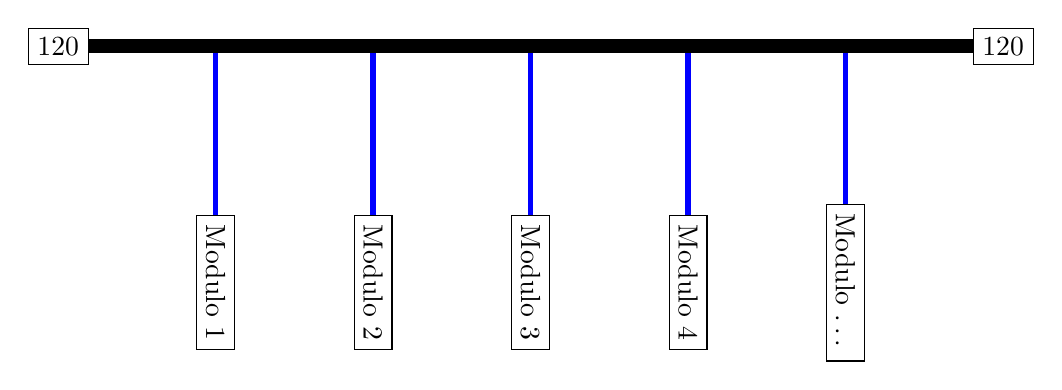
\begin{tikzpicture}
        %\draw [very thin, green]  (-6,-3) grid (6,3);
        \node at (-6,3) [rectangle,draw,align=left] (ps) {\SI{120}{\ohm}};
        \node at (6,3) [rectangle,draw,align=left] (ns) {\SI{120}{\ohm}};
        
        \node at (-4,0) [rectangle,draw,align=left,rotate=-90] (d1) {Modulo 1};
        \node at (-2,0) [rectangle,draw,align=left ,rotate=-90] (d2) {Modulo 2};
        \node at (0,0) [rectangle,draw,align=left ,rotate=-90] (d3) {Modulo 3};

\node at (2,0) [rectangle,draw,align=left ,rotate=-90] (d4) {Modulo 4};

\node at (4,0) [rectangle,draw,align=left ,rotate=-90] (d5) {Modulo \dots};

        \draw [line width=2, blue] (-4,3) --(d1.west);
        \draw [line width=2, blue] (-2,3) --(d2.west);
        \draw [line width=2, blue] (0,3) --(d3.west);

\draw [line width=2, blue] (2,3) --(d4.west);
\draw [line width=2, blue] (4,3) --(d5.west);

        \draw [line width=5] (ps.east) -- (ns.west);
    \end{tikzpicture}
    \caption{Topologia Bus}
    \label{fig:BusPuro}
\end{figure}
Pero a su vez permite algunas ramificaciones siempre y cuando la resitencia entre los conductores diferenciales sea aproximadamente \SI{60}{\ohm}. Ya que todos los modulos estaran conectados en paralelo a los 4 conductores.

\subsection{Segmento - Segmento}


\subsection{Placa - Latiguillo}
Para conectar las placas al bus CBUS tenemos varias opciones validas, y las usaremos segun nos sea util

\subsubsection{Poca Potencia/MERG Screw Terminal Block}
Para las placas de poca potencia (consumo del bus <\SI{100}{\milli\ampere}, o con su propia fuente) podemos usar la solucion de MERG con un bloque terminal tipo MKDS - PHOENIX CONTACT.

El cable a utilizar es el de latiguillo (\SI{0,25}{\milli\metre\squared}/22AWG) usando una ferrula adecuada (Codigo-color). 

\begin{mdframed}
Nota: Sale mas barato comprar 2 de 1x02 que 1 de 1x04 
\end{mdframed}

Tabla de refencias 

\subsection{Media Potencia/MERG Plug Terminal Block}
Cuando la placa requiera mas potencia (Consumo del bus <\SI{500}{\milli\ampere}, ej: esp32 usando Wifi activamente)  podremos usar una version plug 3,5mm o 5mm

Si es posible utilizar el cable de latiguillo (\SI{0,25}{\milli\metre\squared}/22AWG) usando una ferrula adecuada (Codigo), pero si no se puede usar el del bus general
(\SI{0,5}{\milli\metre\squared}/20AWG) con su ferrula adecuada (codigo-color). 

Tabla de refencias 
\subsubsection{Alta Potencia}
Finalmente si la placa requiere mucha potencia, como puede ser un distribuidor de CBUS, o un motor alimentado del bus. Se podra usar la version PCB del conector Cable-Cable o soldar directamente el cable a la PCB

